\subsubsection{Module 5: Tích hợp AI Hỗ trợ Sáng tạo}
Đây là tính năng điểm nhấn của dự án, sử dụng Google Gemini API để hỗ trợ người dùng và người bán tạo nội dung đa phương thức chất lượng cao một cách tự động, bao gồm văn bản, hình ảnh và video ngắn. Hệ thống áp dụng pipeline \textbf{Evaluate--Refine Loop}: sau khi gọi API tạo nội dung, kết quả được đánh giá tự động theo các tiêu chí chất lượng (thang điểm 1--10, ngưỡng chấp nhận $\geq$ 7.0). Nếu chưa đạt, hệ thống tự động sửa prompt và thử lại (tối đa 3 lần) trước khi trả kết quả tốt nhất kèm gợi ý chỉnh sửa cho người dùng.

\begin{figure}[H]
\centering
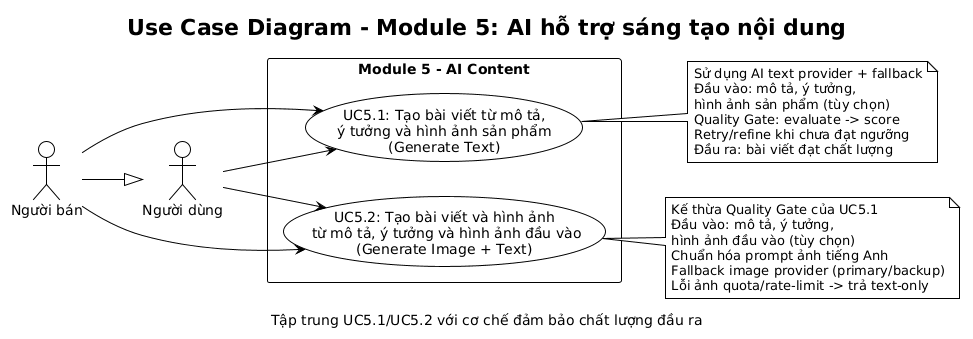
\includegraphics[width=\textwidth]{Images/Usecases/UC-M5-AI.png}
\caption{Sơ đồ Use Case cho Module 5: Tích hợp AI Hỗ trợ Sáng tạo}
\label{fig:usecase-module5}
\end{figure}

\renewcommand{\arraystretch}{1.3}

% UC5.1: GENERATE TEXT
\begin{longtable}{|p{3.5cm}|p{11cm}|}
\caption{Đặc tả Use Case AI Generate Text} \label{tab:uc5.1} \\
\hline
\endfirsthead

\multicolumn{2}{c}%
{{\bfseries \tablename\ \thetable{} -- tiếp tục từ trang trước}} \\
\hline
\endhead

\hline \multicolumn{2}{|r|}{{Tiếp tục ở trang sau}} \\ \hline
\endfoot

\hline
\endlastfoot

\textbf{Tên Use Case} & \textbf{UC5.1: Tạo bài viết từ mô tả, ý tưởng và hình ảnh sản phẩm (Generate Text)} \\ \hline
\textbf{Tác nhân} & Người dùng, Người bán \\ \hline
\textbf{Mô tả} & Cho phép người dùng tạo ra một bài viết hoàn chỉnh dựa trên mô tả, ý tưởng và hình ảnh sản phẩm (nếu có) sử dụng Google Gemini API, với quy trình đánh giá chất lượng tự động và cải thiện prompt khi kết quả chưa đạt. \\ \hline
\textbf{Kích hoạt} & Khi đang soạn thảo bài đăng, người dùng nhấn vào tùy chọn ``Tạo bài viết với AI''. \\ \hline
\textbf{Điều kiện tiên quyết} & 
\begin{itemize}
    \item Người dùng đã đăng nhập và đang trong giao diện tạo bài đăng.
    \item Người dùng đã nhập ít nhất một mô tả hoặc ý tưởng, có thể kèm theo hình ảnh sản phẩm.
\end{itemize} \\ \hline
\textbf{Điều kiện sau} & Một nội dung bài viết hoàn chỉnh (tiêu đề, nội dung, hashtags, CTA) được tạo ra và chèn vào trình soạn thảo, kèm theo điểm đánh giá chất lượng và gợi ý chỉnh sửa (nếu có). \\ \hline
\textbf{Luồng sự kiện chính} & 
\begin{enumerate}
    \item Người dùng nhập mô tả hoặc ý tưởng về bài viết (có thể tải lên hình ảnh sản phẩm).
    \item Người dùng nhấn nút ``Tạo bài viết với AI''.
    \item Hệ thống phân tích đầu vào: trích xuất thực thể chính (tên sản phẩm, đặc điểm, lợi ích), xác định giọng điệu và loại nội dung. Nếu có hình ảnh, phân tích nội dung hình ảnh bằng Gemini Vision.
    \item Hệ thống xây dựng prompt có cấu trúc gồm 5 phần: System Instruction (vai trò chuyên gia nội dung), Context (thông tin thương hiệu, nền tảng), User Input (mô tả + phân tích hình ảnh), Constraints (độ dài 100--300 từ, 5--10 hashtag, phải có CTA), Output Format (JSON schema).
    \item Hệ thống gửi prompt đến Google Gemini API và nhận kết quả.
    \item Hệ thống đánh giá chất lượng kết quả theo 6 tiêu chí có trọng số: Tính liên quan (0.25), Tính hấp dẫn (0.20), Cấu trúc hoàn chỉnh (0.15), Độ dài phù hợp (0.10), Chất lượng ngôn ngữ (0.15), Giá trị thương mại (0.15). Điểm tổng hợp là trung bình có trọng số.
    \item Nếu điểm $\geq$ 7.0/10: hệ thống hiển thị kết quả kèm điểm đánh giá. Nếu điểm $<$ 7.0 và chưa đạt giới hạn 3 lần thử: hệ thống xác định tiêu chí yếu nhất, bổ sung ràng buộc tương ứng vào prompt và gọi lại API (quay lại bước 5). Nếu đã hết lần thử: trả kết quả tốt nhất kèm gợi ý chỉnh sửa.
    \item Hệ thống hiển thị nội dung trong trình soạn thảo kèm điểm đánh giá chi tiết từng tiêu chí và gợi ý cải thiện.
\end{enumerate} \\ \hline
\textbf{Luồng thay thế} & 
\begin{itemize}
    \item A1: Người dùng không hài lòng với kết quả và nhấn ``Tạo lại'' để pipeline chạy lại từ đầu với prompt mới.
    \item A2: Người dùng chỉnh sửa trực tiếp nội dung trong editor (sửa tiêu đề, nội dung, thêm/bớt hashtag).
    \item A3: Người dùng chọn ``Viết lại đoạn này'' để AI viết lại chỉ đoạn được chọn với hướng dẫn cụ thể.
    \item A4: Người dùng thay đổi giọng điệu (chuyên nghiệp, thân thiện, hài hước, sang trọng) và yêu cầu AI viết lại theo giọng điệu mới.
\end{itemize} \\ \hline
\textbf{Ngoại lệ} & 
\begin{itemize}
    \item E1: Lỗi kết nối đến Gemini API $\rightarrow$ Hệ thống báo lỗi ``Không thể tạo nội dung lúc này, vui lòng thử lại sau''.
    \item E2: Hình ảnh không hợp lệ hoặc quá lớn $\rightarrow$ Hệ thống báo lỗi và yêu cầu tải lại hình ảnh.
    \item E3: Gemini API trả về nội dung vi phạm chính sách $\rightarrow$ Hệ thống lọc và yêu cầu tạo lại với prompt đã điều chỉnh.
\end{itemize} \\ \hline
\textbf{Ghi chú} & Pipeline sử dụng chính Gemini API để đánh giá chất lượng (meta-evaluation), kết hợp kiểm tra quy tắc tự động cho các tiêu chí có thể đo lường (format, length, hashtag count). Điểm đánh giá được hiển thị cho người dùng dưới dạng trực quan (thanh tiến trình hoặc biểu đồ radar). \\ \hline
\end{longtable}

% UC5.2: GENERATE IMAGE + TEXT
\begin{longtable}{|p{3.5cm}|p{11cm}|}
\caption{Đặc tả Use Case AI Generate Image + Text} \label{tab:uc5.2} \\
\hline
\endfirsthead

\multicolumn{2}{c}%
{{\bfseries \tablename\ \thetable{} -- tiếp tục từ trang trước}} \\
\hline
\endhead

\hline \multicolumn{2}{|r|}{{Tiếp tục ở trang sau}} \\ \hline
\endfoot

\hline
\endlastfoot

\textbf{Tên Use Case} & \textbf{UC5.2: Tạo bài viết và hình ảnh từ mô tả, ý tưởng và hình ảnh đầu vào (Generate Image + Text)} \\ \hline
\textbf{Tác nhân} & Người dùng, Người bán \\ \hline
\textbf{Mô tả} & Cho phép người dùng tự động tạo ra bài viết kèm hình ảnh dựa trên mô tả, ý tưởng và hình ảnh đầu vào (nếu có) sử dụng Google Gemini API, với đánh giá chất lượng riêng biệt cho text và image. \\ \hline
\textbf{Kích hoạt} & Khi đang soạn thảo bài đăng, người dùng nhấn vào tùy chọn ``Tạo bài viết và hình ảnh với AI''. \\ \hline
\textbf{Điều kiện tiên quyết} & 
\begin{itemize}
    \item Người dùng đã đăng nhập và đang trong giao diện tạo bài đăng.
    \item Người dùng đã nhập ít nhất một mô tả hoặc ý tưởng, có thể kèm theo hình ảnh đầu vào.
\end{itemize} \\ \hline
\textbf{Điều kiện sau} & Một bài viết hoàn chỉnh kèm hình ảnh được tạo bởi AI, cả hai đều được chèn vào trình soạn thảo kèm điểm đánh giá riêng biệt. \\ \hline
\textbf{Luồng sự kiện chính} & 
\begin{enumerate}
    \item Người dùng nhập mô tả hoặc ý tưởng (có thể tải lên hình ảnh đầu vào để tham khảo).
    \item Người dùng nhấn nút ``Tạo bài viết và hình ảnh với AI''.
    \item Hệ thống phân tích đầu vào (tương tự UC5.1), bổ sung phân tích phong cách hình ảnh (màu sắc chủ đạo, bố cục, đối tượng trong ảnh đầu vào).
    \item Hệ thống xây dựng prompt kép: prompt text (5 phần như UC5.1) và prompt image (System Instruction, Context từ text đã tạo, Visual Spec, Constraints về tỷ lệ 1:1/4:5, Negative Prompt).
    \item Hệ thống tạo text trước (với Evaluate--Refine Loop cho text), sau đó sử dụng text đã tạo làm context để tạo image (với Evaluate--Refine Loop riêng cho image).
    \item Đánh giá text: 6 tiêu chí (như UC5.1). Đánh giá image: 4 tiêu chí -- Tính liên quan (0.30), Chất lượng kỹ thuật (0.25), Tính thẩm mỹ (0.25), Nhất quán thương hiệu (0.20). Mỗi loại phải đạt $\geq$ 7.0/10.
    \item Nếu chỉ text hoặc chỉ image chưa đạt: hệ thống chỉ tạo lại phần chưa đạt, giữ nguyên phần đã tốt.
    \item Hệ thống hiển thị bài viết và hình ảnh kèm điểm đánh giá riêng cho từng loại.
\end{enumerate} \\ \hline
\textbf{Luồng thay thế} & 
\begin{itemize}
    \item A1: Người dùng nhấn ``Tạo lại'' để pipeline chạy lại từ đầu.
    \item A2: Người dùng chỉnh sửa text hoặc thay thế hình ảnh riêng biệt.
    \item A3: Người dùng chọn phong cách hình ảnh khác (photorealistic, illustration, flat design) và yêu cầu tạo lại chỉ hình ảnh.
    \item A4: Người dùng tải lên hình ảnh thay thế từ thiết bị, chỉ sử dụng text do AI tạo.
    \item A5: Người dùng yêu cầu AI chỉnh sửa hình ảnh cụ thể (thay đổi màu nền, thêm/bớt đối tượng).
\end{itemize} \\ \hline
\textbf{Ngoại lệ} & 
\begin{itemize}
    \item E1: Lỗi kết nối đến Gemini API $\rightarrow$ Hệ thống báo lỗi ``Không thể tạo nội dung lúc này, vui lòng thử lại sau''.
    \item E2: Gemini API không thể tạo hình ảnh phù hợp sau 3 lần thử $\rightarrow$ Hệ thống trả về bài viết kèm thông báo và gợi ý chỉnh sửa prompt hình ảnh.
    \item E3: Hình ảnh đầu vào không hợp lệ $\rightarrow$ Hệ thống báo lỗi và yêu cầu tải lại hình ảnh.
\end{itemize} \\ \hline
\textbf{Ghi chú} & Hai Evaluate--Refine Loop chạy tuần tự (text trước, image sau) để đảm bảo hình ảnh phù hợp với nội dung text. Chỉ phần chưa đạt ngưỡng mới được tạo lại, tối ưu chi phí gọi API. \\ \hline
\end{longtable}

% UC5.3: GENERATE VIDEO + IMAGES + TEXT
\begin{longtable}{|p{3.5cm}|p{11cm}|}
\caption{Đặc tả Use Case AI Generate Video + Images + Text} \label{tab:uc5.3} \\
\hline
\endfirsthead

\multicolumn{2}{c}%
{{\bfseries \tablename\ \thetable{} -- tiếp tục từ trang trước}} \\
\hline
\endhead

\hline \multicolumn{2}{|r|}{{Tiếp tục ở trang sau}} \\ \hline
\endfoot

\hline
\endlastfoot

\textbf{Tên Use Case} & \textbf{UC5.3: Tạo video ngắn, hình ảnh và bài viết từ mô tả, ý tưởng và hình ảnh đầu vào (Generate Video + Images + Text)} \\ \hline
\textbf{Tác nhân} & Người dùng, Người bán \\ \hline
\textbf{Mô tả} & Tính năng AI nâng cao nhất, tạo bài đăng đa phương thức (video ngắn + tối đa 3 hình ảnh + bài viết) với pipeline đánh giá ba tầng độc lập, sử dụng Google Gemini API và Google Veo 2. \\ \hline
\textbf{Kích hoạt} & Khi đang soạn thảo bài đăng, người dùng nhấn vào tùy chọn ``Tạo video và nội dung đa phương thức với AI''. \\ \hline
\textbf{Điều kiện tiên quyết} & 
\begin{itemize}
    \item Người dùng đã đăng nhập và đang trong giao diện tạo bài đăng.
    \item Người dùng đã nhập ít nhất một mô tả hoặc ý tưởng, có thể kèm theo hình ảnh đầu vào.
\end{itemize} \\ \hline
\textbf{Điều kiện sau} & Một bài đăng đa phương thức hoàn chỉnh (video + images + text) kèm điểm đánh giá từng loại được chèn vào trình soạn thảo. \\ \hline
\textbf{Luồng sự kiện chính} & 
\begin{enumerate}
    \item Người dùng nhập mô tả hoặc ý tưởng (có thể tải lên hình ảnh đầu vào).
    \item Người dùng nhấn nút ``Tạo video và nội dung đa phương thức với AI''.
    \item Hệ thống phân tích đầu vào (tương tự UC5.2), bổ sung xác định storyboard concept (cảnh mở đầu, giới thiệu, highlight, CTA).
    \item Hệ thống thực hiện pipeline tuần tự ba tầng:
    \begin{itemize}
        \item \textbf{Tầng 1 -- Text}: Xây dựng prompt text $\rightarrow$ Gemini API $\rightarrow$ Đánh giá 6 tiêu chí $\rightarrow$ Evaluate--Refine Loop (tối đa 3 lần).
        \item \textbf{Tầng 2 -- Images}: Dùng text làm context $\rightarrow$ Xây dựng prompt image $\rightarrow$ Gemini API tạo tối đa 3 ảnh $\rightarrow$ Đánh giá 4 tiêu chí mỗi ảnh $\rightarrow$ Evaluate--Refine Loop.
        \item \textbf{Tầng 3 -- Video}: Dùng text + images làm context $\rightarrow$ Tự động tạo storyboard $\rightarrow$ Xây dựng prompt video (15--30 giây, tỷ lệ 9:16/1:1) $\rightarrow$ Google Veo 2 $\rightarrow$ Đánh giá 5 tiêu chí: Tính mạch lạc (0.25), Chất lượng hình ảnh (0.25), Độ dài phù hợp (0.15), Tính hấp dẫn (0.20), Nhất quán nội dung (0.15) $\rightarrow$ Evaluate--Refine Loop.
    \end{itemize}
    \item Mỗi tầng Evaluate--Refine Loop chạy độc lập. Khi tạo lại tầng sau, kết quả tầng trước đã đạt được giữ nguyên.
    \item Hệ thống hiển thị video, hình ảnh và bài viết kèm điểm đánh giá chi tiết từng loại. Người dùng có thể chỉnh sửa hoặc tạo lại riêng từng thành phần.
\end{enumerate} \\ \hline
\textbf{Luồng thay thế} & 
\begin{itemize}
    \item A1: Người dùng nhấn ``Tạo lại'' toàn bộ để pipeline chạy lại từ đầu.
    \item A2: Người dùng tạo lại chỉ một thành phần (ví dụ: chỉ video) với yêu cầu bổ sung.
    \item A3: Người dùng chỉnh sửa text, thay thế hình ảnh hoặc video trước khi đăng.
    \item A4: Người dùng cung cấp storyboard chi tiết hơn để cải thiện chất lượng video.
    \item A5: Người dùng chỉ sử dụng một phần nội dung (ví dụ: text + images, bỏ video).
\end{itemize} \\ \hline
\textbf{Ngoại lệ} & 
\begin{itemize}
    \item E1: Lỗi kết nối đến Gemini API hoặc Google Veo 2 $\rightarrow$ Hệ thống báo lỗi.
    \item E2: Gemini API không thể tạo video phù hợp sau 3 lần thử $\rightarrow$ Hệ thống trả về images + text kèm gợi ý cải thiện prompt video.
    \item E3: Hình ảnh đầu vào không hợp lệ $\rightarrow$ Hệ thống báo lỗi.
    \item E4: Video vượt quá 30 giây $\rightarrow$ Kiểm tra rule-based đánh trượt, tự động tạo lại với ràng buộc thời lượng chặt hơn.
\end{itemize} \\ \hline
\textbf{Ghi chú} & Pipeline ba tầng đảm bảo tính nhất quán: text làm nền tảng cho images, text + images làm nền tảng cho video. Đánh giá ``Nhất quán nội dung'' (tiêu chí video) kiểm tra phong cách video có khớp với images và text đã tạo. \\ \hline
\end{longtable}